% !TeX spellcheck = en_GB
\documentclass[10pt,letterpaper,oneside]{article}
\usepackage{fontspec}
\usepackage{arev}
\usepackage[utf8]{inputenc}
\usepackage[T1]{fontenc}
\usepackage{amsmath}
\usepackage{amsfonts}
\usepackage{amssymb}
\usepackage{graphicx}
\usepackage{csquotes}
\usepackage{booktabs}
\usepackage{multicol}
\usepackage{enumerate}
\usepackage{microtype}
\usepackage[labelfont=bf,font={small}]{caption}
\usepackage{hyperref}
\usepackage{booktabs}
\usepackage{subcaption}
\usepackage{fancyhdr}
\usepackage[svgnames]{xcolor}
\usepackage{mdframed}
\usepackage{multicol}
\usepackage[para]{footmisc}
\usepackage{siunitx}
\usepackage{cleveref}
\usepackage{listings}
\usepackage{cprotect}


\lstset{ % General setup for the package
	language=Python,
	basicstyle=\small\ttfamily,
	tabsize=4,
	columns=fixed,
	showstringspaces=false,
	showtabs=false,
	keepspaces,
	commentstyle=\color{SeaGreen},
	keywordstyle=\bf\ttfamily\color{DarkBlue}
}

\newfontfamily\symbolfont{Symbola}
\usepackage[left=1in,right=1in,top=1in,bottom=1in,marginparwidth=0.3in]{geometry}

\usepackage[sorting=none]{biblatex}
\addbibresource{../bibliography.bib}

\author{Andreas Stöckel\\[0.5cm]Based on lecture notes by\\Chris Eliasmith and Terrence~C.~Stewart}
\newcommand{\baseCodeURL}{https://github.com/astoeckel/syde556-w20/blob/master/lectures}

\fancyhf{}
\fancyhead[L]{SYDE 556/750 Lecture Notes}
\fancyhead[R]{Andreas Stöckel}
\fancyfoot[C]{\thepage}
\pagestyle{fancy}

\setlength{\parindent}{0em}
\setlength{\parskip}{0.5em}
\renewcommand{\baselinestretch}{1.25}
\renewcommand{\vec}[1]{{\mathbf{#1}}}
\newcommand{\mat}[1]{{\mathbf{#1}}}
\newcommand{\T}{\ensuremath{\mathrm{T}}}
\renewcommand{\epsilon}{\varepsilon}
\renewcommand{\phi}{\varphi}

\makeatletter
\newcommand{\superimpose}[2]{%
	{\ooalign{{#1}\hidewidth\cr{#2}\hidewidth\cr}}}
\makeatother
\newcommand{\SolidCircle}[2]{\superimpose{\color{#1}\symbolfont ⬤}{\textbf{\color{white}#2}}\hspace{1em}}
\newcommand{\OPlus}{\SolidCircle{DarkGreen}{\kern0.75pt+}}
\newcommand{\OMeh}{\SolidCircle{DarkOrange}{~}}
\newcommand{\OMinus}{\SolidCircle{DarkRed}{\kern2.25pt--}}

\newcommand{\YouTube}[2][Video]{\href{https://youtu.be/#2}{{\symbolfont 📺}~{#1}}%
%\footnote{\url{https://youtu.be/#2}}%
}

\newcommand{\CodeLink}[2][Code]{\href{\baseCodeURL/#2}{{\symbolfont ⌨}~\emph{#1}}}

\newcommand{\MakeTitle}[1]{
\maketitle
\begin{center}
	
\includegraphics[width=0.5\textwidth]{../assets/uwlogo.pdf}\\[1cm]
	{#1}\
\end{center}

\vfill

\thispagestyle{empty}
\setcounter{page}{0}
\newpage

\pagenumbering{roman}
\setcounter{tocdepth}{2}
\tableofcontents
\newpage

\setcounter{page}{0}
\pagenumbering{arabic}}

\reversemarginpar


\newcommand{\ColorBox}[3]{%
	\marginpar{%
		\huge\raisebox{-3ex}{\symbolfont{#1}}%
	}%
	\begin{mdframed}[hidealllines=true,backgroundcolor=#2,innertopmargin=0.25cm,innerbottommargin=0.25cm]%
		{#3}
	\end{mdframed}}

\newcommand{\Note}[1]{\ColorBox{📌}{WhiteSmoke}{\textbf{Note:} #1}}
\newcommand{\Example}[1]{\ColorBox{💡}{WhiteSmoke}{\textbf{Example:} #1}}
\newcommand{\Aside}[1]{\ColorBox{🌟}{WhiteSmoke}{\emph{Aside:} #1}}
\newcommand{\Python}[1]{\ColorBox{🐍}{WhiteSmoke}{#1}}
\newcommand{\Notation}[1]{\ColorBox{\huge$\Sigma$}{WhiteSmoke}{\textbf{Notaton:} #1}}

\newcommand{\ConstructionSite}{\hrulefill {\symbolfont 🚧} UNDER CONSTRUCTION {\symbolfont 🚧} \hrulefill}

\newenvironment{ImportantEqn}[1]{\mdframed\raggedleft\emph{({#1})}\align}{\endalign\endmdframed}

\date{January 9, 2020}
\title{SYDE 556/750 \\ Simulating Neurobiological Systems \\ Lecture 2: Neurons}


\begin{document}

\MakeTitle{\textbf{Accompanying Readings: Chapter 4.1 of Neural Engineering}}

\section{Introduction}

\Note{In the last lecture, we took a deep dive into neuroscience, and we saw how \enquote{messy} and complex nervous systems are. In this lecture we try to back up a little, moving us back to the safe haven of mathematical abstraction.}

\begin{figure}[b]
	\centering
	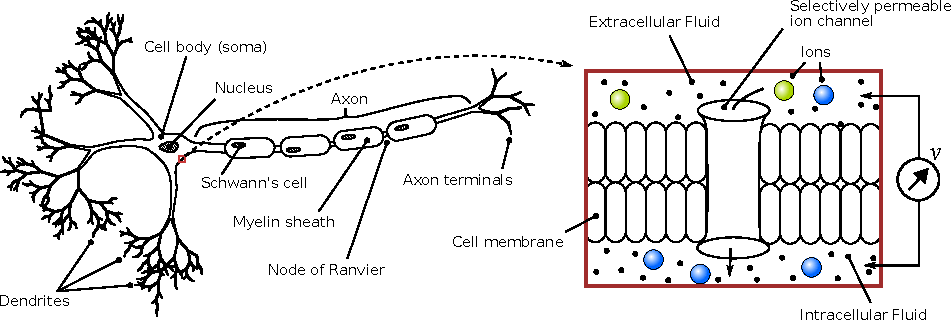
\includegraphics{media/neuron_sketch_membrane.pdf}
	\caption{Illustration showing a text-book neuron, as well as a schematic cross-section through the cell membrane. Left part of the illustration from \cite{stoeckel2015design}, adapted from \cite{kandel2012principles}.}
	\label{fig:neuron_sketch_membrane}
\end{figure}

Neurons are the fundamental unit of computation in the nervous system. They compute by receiving action potentials (spikes) from pre-synaptic neurons in their dendrites. In most neurons, once the number of spikes received within a certain timespan surpasses a threshold, the neuron itself may emit an action potential that is being propagated along the neuron's axon to the axon terminal, where it will pass across a synapse to the post-neuron's dendrites where the process repeats (cf.~\cref{fig:neuron_sketch_membrane}).

From an engineering perspective, we could say that individual neurons exchange coded information. An important part of understanding nervous systems is thus to understand the \enquote{code} that is being used for neural communication.

Unfortunately, there is no scientific consensus as for what exactly this \enquote{neural code} is. Most evidence points at a combination of population coding (i.e.,~information is encoded in the relative activities of a group of neurons) and time coding (i.e.,~the timing of individual spikes matters) \cite{rieke1999spikes}.

\Note{There isn't a single neural code; different coding strategies are employed in different parts of the nervous system. Codes differ significantly between the peripheral nervous system (i.e.,~the sensory and motor neurons distributed throughout the body; especially the latter are clearly using a rate code) and the central nervous system.}

What we do have however, are detailed models that describe how individual neurons generate action potentials. Thus, we will approach the problem of deciphering the neural code in two stages. First, in this lecture, we will have a look at single neurons and try to get an understanding of how neurons generate action potentials. We discuss the so called \enquote{Leaky Integrate-and-Fire} neuron, and summarize its behaviour in a simple analytical expression. Second, in the next two lectures, we think about the neural code in terms of \emph{neural representation}, which will lead us to a theory that predicts what the neural code may be.

\section{Spiking Neurons}

\Note{We're going to have a slightly closer look at biologically detailed spiking neuron models towards the end of the term. For now, we're skimming over the details. Have a look at \cite{kandel2012principles} (particularly Chapter 7 and 8) if you want to learn more about basic neurobiology.}

Neurons are cells that specialise in the integration and transmission of electrical signals. Cells in general are separated from the environment by a thick, impermeable \enquote{barrier}, the \emph{cell membrane}, consisting of a bi-layer of lipid molecules. The cell membrane establishes an \enquote{intracellular} space that is isolated from the \enquote{extracellular} space. Both spaces are filled with a watery liquid, called the \emph{intracellular fluid} and \emph{extracellular fluid}, respectively (\cref{fig:neuron_sketch_membrane}).

\subsection{Qualitative neural behaviour}

When we insert an electrode into a resting neuron (akin to the \enquote{single electrode recording} we saw earlier), we can measure a difference in electrical potential, i.e.,~a voltage $v$, between the intra- and extracellular space (\cref{fig:neuron_sketch_membrane}). We call this voltage the \emph{resting potential} $E_\mathrm{L}$.\footnote{The symbol \enquote{$E_\mathrm{L}$} stems from the alternative name of this potential, the \enquote{\textbf{L}eak channel \textbf{E}quilibrium potential}.}

Instead of just measuring this potential, we may also inject an external current into the neuron by hooking it up to a current source (i.e.,~a precision power supply that controls current instead of voltage). This is similar to what happens whenever a neuron receives a spike from a pre-synaptic neuron: the synapse induces either a positive (\enquote{excitatory synapse}), or a negative (\enquote{inhibitory synapse}) current that flows into the neuron.

\begin{figure}
	\centering%
	\begin{subfigure}{0.5\textwidth}%
		\centering
		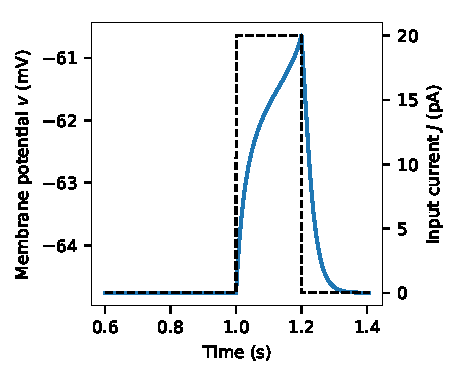
\includegraphics{media/hh_neuron_sub_threshold.pdf}%
		\caption{Sub-threshold neuron}%
		\label{fig:hh_neuron_sub_threshold}
	\end{subfigure}%
	\begin{subfigure}{0.5\textwidth}%
		\centering
		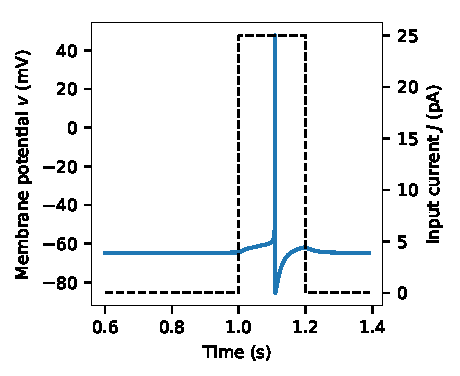
\includegraphics{media/hh_neuron_super_threshold.pdf}%
		\caption{Super-threshold neuron}%
		\label{fig:hh_neuron_super_threshold}
	\end{subfigure}%
	\caption{Computer simulation of a Hodgkin Huxley type model neuron \cite{hodgkin1952quantitative,traub1991neuronal}. The blue line corresponds to the membrane potential $v$, the dashed line to the current $J$ that is being injected into the neuron. The time axis starts at \SI{0.6}{\second} to make sure that the neuron has settled into its resting state. \CodeLink[Code (simulation)]{lecture_02/media/code/hh_neuron.cpp}, \CodeLink[Code (plotting)]{lecture_02/media/code/hh_neuron_plot.ipynb}}
\end{figure}

When injecting positive (\enquote{excitatory}) currents into a neuron, we observe four major things:
\begin{enumerate}
	\item The cell acts like a \emph{capacitor}, i.e., the voltage increases while we're injecting a current (\cref{fig:hh_neuron_sub_threshold}).
	\item The capacitor is \emph{leaky}. As soon as we stop injecting a current, the voltage collapses back to the resting potential $E_\mathrm{L}$ (\cref{fig:hh_neuron_sub_threshold}).
	\item As soon as the voltage surpasses a certain value, the \emph{threshold potential} $v_\mathrm{th}$, the cell will generate a spike (\cref{fig:hh_neuron_super_threshold}).
	\item Shortly after the spike has been produced, the voltage drops below the resting potential. During this period, the \emph{refractory period} of length $\tau_\mathrm{ref}$, we cannot get the neuron to spike again, even if we apply relatively large input currents $J$ (\cref{fig:hh_neuron_super_threshold}).
\end{enumerate}

\newpage

\Note{Importantly, neurons in biology are \emph{dynamical systems}, i.e., they possess a behaviour that evolves over time. \emph{Artificial neurons} in machine learning (see below) are time-independent. They are mathematical functions that take an input that is \enquote{immediately} being mapped onto an output.}

\subsection{The Leaky Integrate and Fire Neuron}

We can qualitatively summarize this behaviour in a very simple model, the so called \enquote{Leaky Integrate and Fire} neuron model. This model was first proposed by the French scientist Louis Lapicque in 1907 \cite{lapicque1907recherches,abbott1999lapicque}.

\paragraph{Sub-threshold behaviour}
First, we have the \emph{sub-threshold} behaviour, a so called leaky integrator.
\begin{align}
	\begin{aligned}
		\frac{\mathrm{d}}{\mathrm{d}t} v(t) &= \frac{1}{C_\mathrm{m}} \big(g_\mathrm{L} (E_\mathrm{L} - v(t))
			+ J
		\big) \,, \quad \text{if } v(t) < v_\mathrm{th}\,.
	\end{aligned}
	\label{eqn:sub-threshold}
\end{align}
This differential equation corresponds to a capacitor with capacity $C_\mathrm{m}$ that is charged with a current $J$ and that slowly discharges to a potential $v_\mathrm{reset}$ over a resistor with conductance (the inverse of the resistance) $g_\mathrm{L} = \frac{1}{R}$ (the \emph{leak conductance}):
\begin{center}
	\hspace{2.5cm}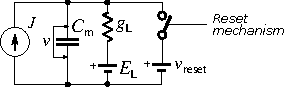
\includegraphics[scale=1.5]{media/lif_circuit.pdf}
\end{center}

\paragraph{Super-threshold behaviour}
Second, we have the \emph{super-threshold behaviour}, i.e.~the spike production and refractory period. Assume $v(t) = v_\mathrm{th}$ at $t = t_\mathrm{th}$. Then
\begin{align}
	\begin{aligned}
		v(t) &\gets \delta(t - t_\mathrm{th}) \,, &\text{if } t &= t_\mathrm{th} \,,\\
		v(t) &\gets v_\mathrm{reset} \,, &\text{if } t &> t_\mathrm{th} \text{ and } t \geq t_\mathrm{th} + \tau_\mathrm{ref} \,,
	\end{aligned}
	\label{eqn:super-threshold}
\end{align}

\Note{$\delta(t)$ is the Dirac delta function, i.e., the function defined as
\begin{align*}
	\delta(t) &= \begin{cases} \infty & \text{if } t = 0 \, \\ 0 & \text{if } t \neq 0 \,, \end{cases}  \quad \text{ and } \quad \int_{-\infty}^\infty \delta(t)\,\mathrm{d}t = 1 \,.
\end{align*}}

\paragraph{Normalized equations}
For our modelling purposes, we don't really care about the exact values of $v_\mathrm{th}$, $v_\mathrm{reset}$ and $E_\mathrm{L}$. We can normalise these voltages, i.e., assume that $v_\mathrm{th} = 1$, and $v_\mathrm{reset} = E_\mathrm{L} = 0$. Now we can simplify \cref{eqn:sub-threshold,eqn:super-threshold} to
\begin{align}
	\begin{aligned}
		\frac{\mathrm{d}}{\mathrm{d}t} v(t) &= -\frac{1}{\tau_\mathrm{RC}} \big( v(t) - RJ \big)
		\big) \,, \quad &\text{if } v(t) &< v_\mathrm{th}\,. \\
		v(t) &\gets \delta(t - t_\mathrm{th}) \,, &\text{if } t &= t_\mathrm{th} \,,\\
v(t) &\gets 0 \,, &\text{if } t &> t_\mathrm{th} \text{ and } t \geq t_\mathrm{th} + \tau_\mathrm{ref} \,,
	\end{aligned}
	\label{eqn:sub-threshold-normalised}
\end{align}
where, $\tau_\mathrm{RC} = C_\mathrm{m} R$ and $R = \frac{1}{g_\mathrm{L}}$.

\subsection{Characterizing the firing-rate of a LIF Neuron}

\begin{figure}[t]
	\begin{subfigure}{\textwidth}
		\centering
		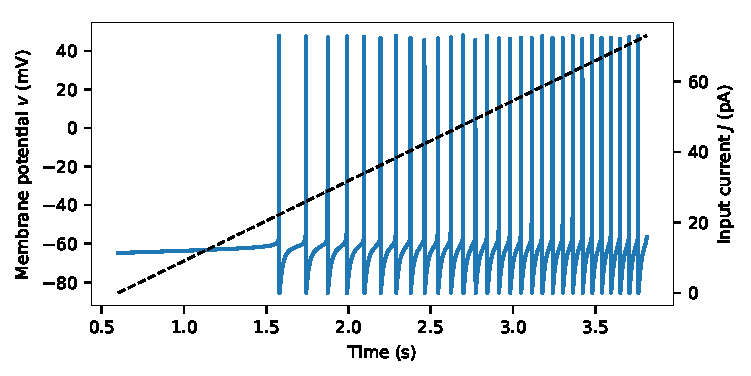
\includegraphics{media/hh_neuron_ramp.pdf}
		\caption{Hodgkin-Huxley model neuron}
	\end{subfigure}
	\begin{subfigure}{\textwidth}
		\centering
		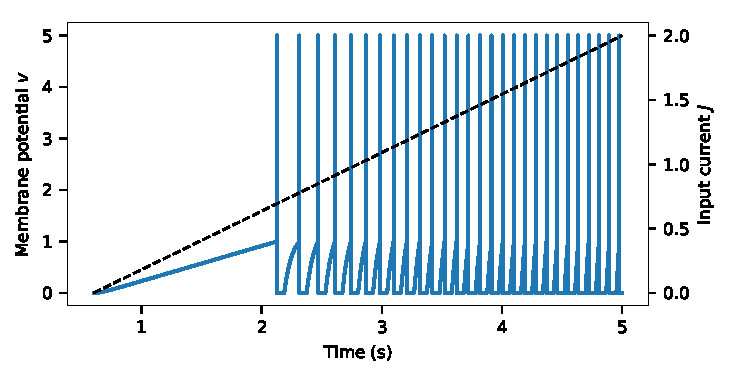
\includegraphics{media/lif_neuron_ramp.pdf}
		\caption{Normalized Leaky Integrate-and-Fire neuron}
	\end{subfigure}
	\caption{Effects of a current ramp on an Hodgkin-Huxley type model neuron and a (normalized) LIF neuron. As above, the blue line is the membrane potential, the dashed line is the input current. \CodeLink[Code (simulation)]{lecture_02/media/code/hh_neuron.cpp}, \CodeLink[Code (plotting)]{lecture_02/media/code/hh_neuron_plot.ipynb}}
	\label{fig:current_ramp}
\end{figure}

\Cref{fig:current_ramp} depicts the behaviour of the LIF neuron model \cref{eqn:sub-threshold-normalised}, as well as the detailed Hodgkin-Huxley type neuron model from before, as we slowly increase the input current $J$. Overall, we can see that the behaviour of the LIF neuron matches the behaviour of the more complex model quite well -- at least qualitatively speaking.

Furthermore, we observe that the neurons fire quite regularly, yet the rate at which each neuron emits spikes (is \enquote{firing}) increases as we increase the input current.

This raises the question: instead of dealing with these complicated differential equations, could we just summarize the behaviour of the neuron, e.g.,~compute the \emph{firing rate} $a$ for a given input current $J$? At least for the LIF neuron we can derive an analytic expression $G[J]$, the so called \emph{neural response curve} that maps a current $J$ onto the average spikes per second.

\newpage

\Note{Of course, with this \emph{rate approximation}, we loose any information about spike timing. And having access to spike timing is still very useful when we want to bridge to lower levels of organization. We will deal with this in two weeks, when we talk about \emph{temporal representation}. Furthermore, spiking communication induces \emph{noise} that may be important from a modelling perspective.}

Since the sub-threshold portion of \cref{eqn:sub-threshold-normalised} is a simple first-order linear differential equation we can actually fully characterize the behaviour of the LIF neuron under the assumption of a constant input current. Particularly, we can derive a closed form expression that describes the time $t_\mathrm{th}$ it takes for the threshold potential to be reached and a spike to be produced, assuming that the neuron is in its reset state at $t=0$, $v(0) = 0$. Writing down such an analytic expression is not possible for most -- even slightly more complex -- neuron models.

\paragraph{Computing the time-to-threshold $t_\mathrm{th}$}
To compute $t_\mathrm{th}$, we first need to solve the subthreshold differential equation under the assumption that $J$ is constant and the initial condition is $v(0) = 0$. In general, this differential equation can be solved according to the \enquote{variation of constants} formula
\begin{align*}
	v(t) &= - \int_0^t \frac{1}{\tau_\mathrm{RC}} \big( v(t') - RJ \big) \,\mathrm{d}t'
	      = RJ \left(1 - e^{-\frac{t}{\tau_\mathrm{RC}}} \right) \,.
\end{align*}
For the given assumptions, this equation can be used to compute the membrane potential at any time $t$. Of course, this does not take the super-threshold behaviour into account.

Second, we can compute the point in time $t_\mathrm{th}$ at which the membrane potential will reach $v_\mathrm{th}$:
\begin{align*}
	v_\mathrm{th} &= RJ \left(1 - e^{-\frac{t_\mathrm{th}}{\tau_\mathrm{RC}}} \right) \,, \\
	\Leftrightarrow 1 - \frac{v_\mathrm{th}}{RJ} &= e^{-\frac{t_\mathrm{th}}{\tau_\mathrm{RC}}} \,, && \Big| \, RJ \neq 0 \\
	\Leftrightarrow - \tau_\mathrm{RC} \log \left( 1 - \frac{v_\mathrm{th}}{RJ} \right) &= t_\mathrm{th} \,.  && \Big| \, 1 - \frac{v_\mathrm{th}}{RJ} > 0 , RJ \neq 0
\end{align*}

\Note{The terms right of the \enquote{$|$} specify the conditions for which equivalence holds. It is always useful to remember the conditions under which a derived equation remains valid.}

Note that for $1 - \frac{v_\mathrm{th}}{RJ} < 0$ the input current is so small that the membrane potential will converge to an equilibrium below $v_\mathrm{th}$, and hence $t_\mathrm{th} \to \infty$ -- in other words, the neuron does not spike at all in this case.

\paragraph{Computing the firing rate}

Note that the LIF neuron model assumes that neurons have no \enquote{memory}. Whenever the neuron spikes, it is reset to it's initial state. This means that the LIF neuron response is perfectly periodic as long as the input remains constant.

\Note{The \enquote{no memory} assumption -- and thus the perfect periodicity of the LIF neuron model -- does not hold for other neuron models. However, for any neuron model, we could approximate $G[J]$ numerically by applying the current $J$, simulating the neuron over a time period $T$ and then measuring the number of spikes $n$ over $T$, i.e.,~$G[J] \approx n(J) / T$.}

Given $t_\mathrm{th}$ we can compute the firing rate $G[J]$ of the neuron, i.e.,~the average number of output spikes during one second for a given input current $J$. The firing rate is the inverse of the inter-spike-interval (ISI), which is the sum of $t_\mathrm{th}$ (time-to-fire) and the refractory period $\tau_\mathrm{ref}$:
\begin{align*}
	G[J]
		&= \begin{cases}
			\frac{1}{\tau_\mathrm{ref} + t_\mathrm{th}(J)} & \text{if } 1 - \frac{v_\mathrm{th}}{RJ} > 0 \,,\\
			0 & \mathrm{otherwise} \,,
		\end{cases} \\
		&= \begin{cases}
			\frac{1}{\tau_\mathrm{ref} - \tau_\mathrm{RC} \log \left( 1 - \frac{v_\mathrm{th}}{RJ} \right)} & \text{if } 1 - \frac{v_\mathrm{th}}{RJ} > 0 \,,\\
			0 & \mathrm{otherwise} \,.
		\end{cases}
\end{align*}

Remember that we defined $v_\mathrm{th} = 1$. Furthermore, if we only want to characterize the LIF firing rate qualitatively, we can assume $R = 1$, since this resistance just rescales our input current (note that all variables are now unit-less). This gives us our final equation that fully summarizes the behaviour of the LIF neuron (\cref{fig:lif_neuron_rate}):
\begin{ImportantEqn}{LIF neuron rate approximation}
	G[J]
	&= \begin{cases}
	\frac{1}{\tau_\mathrm{ref} - \tau_\mathrm{RC} \log \left( 1 - \frac{1}{J} \right)} & \text{if } J > 1 \,,\\
	0 & \mathrm{otherwise} \,.
	\end{cases}
\end{ImportantEqn}


\begin{figure}
	\centering%
	\begin{subfigure}{0.5\textwidth}%
		\centering%
		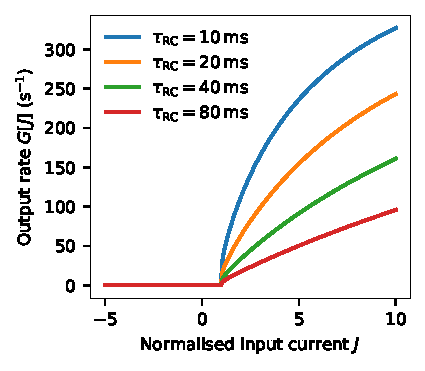
\includegraphics{media/lif_neuron_rate_tau_rc.pdf}%
	\end{subfigure}%
	\begin{subfigure}{0.5\textwidth}%
		\centering%
		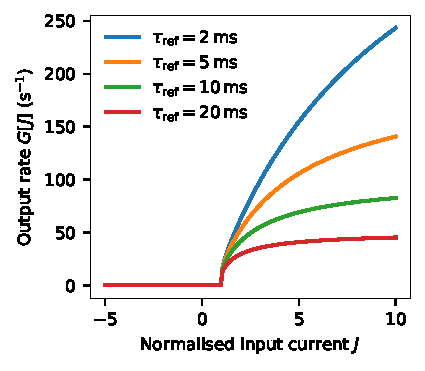
\includegraphics{media/lif_neuron_rate_tau_ref.pdf}%
	\end{subfigure}%
	\caption{LIF rate approximation response curve $G[J]$ for different $\tau_\mathrm{RC}$ and $\tau_\mathrm{ref}$. \CodeLink{lecture_02/media/code/neuron_nonlinearities.ipynb}}
	\label{fig:lif_neuron_rate}
\end{figure}

\subsection{Limitations of the LIF neuron model}

\begin{figure}
	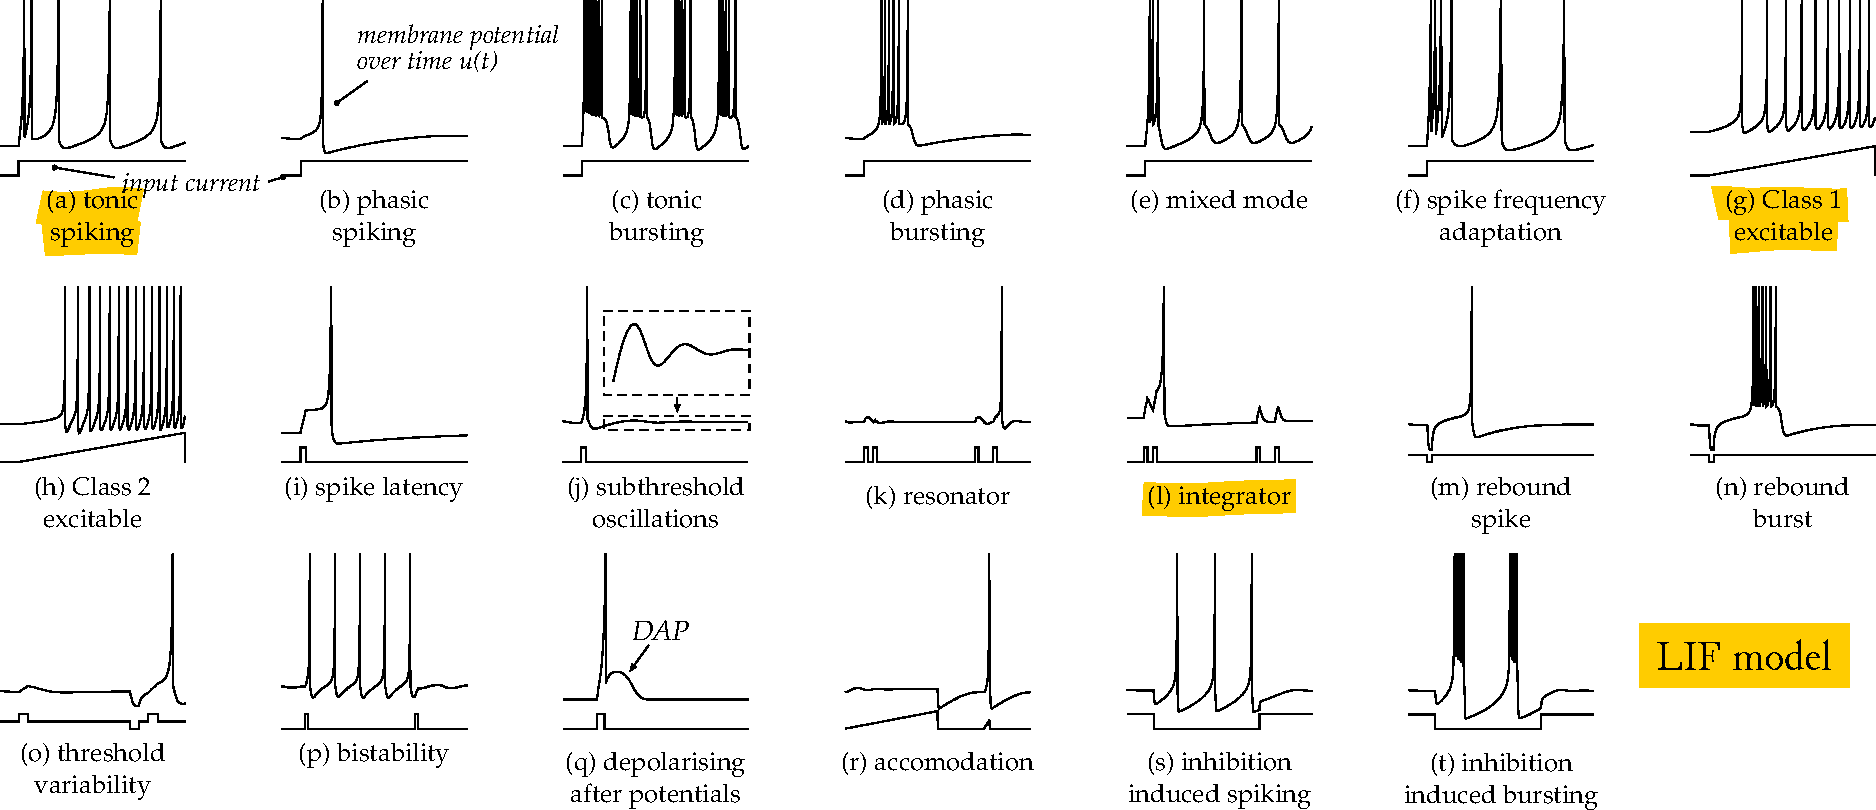
\includegraphics[width=\textwidth]{media/izhikevich_whichmod_figure2.pdf}
	\caption{Single-neuron behaviours observed in nature. The highlighted behaviours correspond to those that are explained by the LIF neuron model. Upper plot of each subfigure corresponds to the membrane potential, lower plot to the input current. Figure from \cite{stoeckel2015design}, adapted from \cite{izhikevich2004model}. All these behaviours can be explained with the slightly more complex (two instead of one state variables) Izhikevich neuron model~\cite{izhikevich2003simple}.}
	\label{fig:izhikevich_whichmod_figure2}
\end{figure}

From looking at \cref{fig:current_ramp}, it may seem as if the LIF neuron model and the biophysically more plausible Hodgkin-Huxley type model exhibit the same qualitative behaviour. In general, this is not true -- this observation only holds for certain sets of neuron parameters and inputs. While the LIF neuron model certainly is a good first-order approximation of neural behaviour, it does not account for some neurophysiological phenomena observed in biology (\cref{fig:izhikevich_whichmod_figure2}).

For various reasons, we are not concerned with these limitations for now. First, as we will see when we talk about temporal representation, the methods we are using are not limited to LIF neurons -- as long as we have a dynamical system description of the neuron we are using, we can compute the connection weights that implement a certain behaviour.

Second, before we add more complexity to our models -- such as the ability to produce the complex neural responses from \cref{fig:izhikevich_whichmod_figure2} -- we should ask ourselves first what the implications for producing high-level behaviour are. In our opinion, it only makes sense to add more detail if this somehow constrains the kind of behaviour our models can produce.

Lastly, many of these phenomena can also be produced by LIF neurons when considering network effects, and not just individual neurons.

\newpage

\Note{As hinted at above, we will talk about more complex neuron models in the NEF at the end of the course, if time permits.}

\section{Artificial \enquote{Rate} Neurons}

Using rate approximations instead of spiking dynamical systems is an idea that gave rise to the artificial neural networks used in machine learning -- neurons are reduced to a function that maps an input (in biology: a current) onto a \enquote{firing rate}. In machine learning, this function is called the \enquote{non-linearity}. Being non-linear is an important aspect of computation in neural systems, since purely linear elements cannot perform any computation -- apart from this, most artifical neuron response functions relatively little to do with actual neural response curves --  more often than not, they are optimized for computationally cheap evaluation and differentiation instead of biological realism. We are mostly going over these nonlinearities as a point for comparison to the LIF rate approximation we just derived.

\Note{As a reminder, here is the definition of what it means for a function to be \emph{linear}.
	
A function $f : \mathbb{R}^m \longrightarrow \mathbb{R}^n$ is linear, \emph{exactly if} the following equality holds
\begin{align*}
	f(a \cdot \vec x + b \cdot \vec y) = a \cdot f(\vec x) + b \cdot f(\vec y) \quad \text{for all } a, b \in \mathbb{R} \text{ and } \vec x, \vec y \in \mathbb{R}^m.
\end{align*}

Another definition that makes use of matrix multiplication is the following.

A function $f : \mathbb{R}^m \longrightarrow \mathbb{R}^n$ is linear, \emph{exactly if} there exists a matrix $\mat F \in \mathbb{R}^n \times \mathbb{R}^m$ such that
\begin{align*}
	f(\vec x) = \mat F \vec x  \quad \text{for all } \vec x \in \mathbb{R}^m\,.
\end{align*}
This implies -- reading the definition in the backwards direction -- that every matrix $\mat A$ defines a corresponding linear function.}

Next, we will take a look at some examples of neural non-linearities (or, in biological terms, \enquote{neural response functions}).

\begin{figure}
	\centering%
	\begin{subfigure}{0.5\textwidth}%
		\centering%
		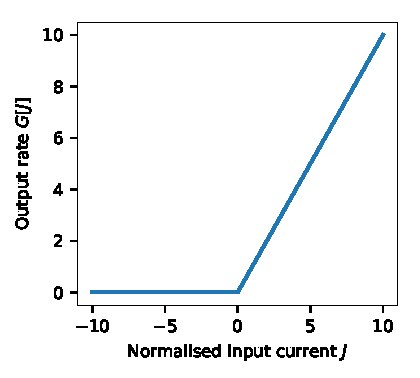
\includegraphics{media/nonlinearity_relu.pdf}%
		\caption{Rectified Liner (ReLU)}%
		\label{fig:artificial_neurons_relu}
	\end{subfigure}%
	\begin{subfigure}{0.5\textwidth}%
		\centering%
		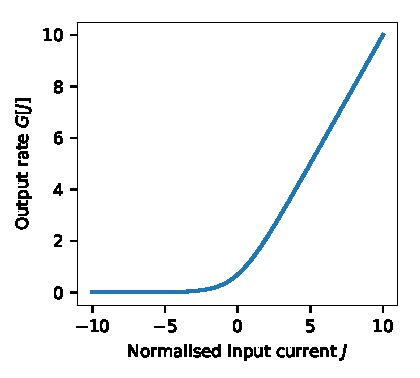
\includegraphics{media/nonlinearity_smooth_relu.pdf}%
		\caption{Soft Rectified linear}%
		\label{fig:artificial_neurons_smooth_relu}
	\end{subfigure}
	\begin{subfigure}{0.5\textwidth}%
		\centering%
		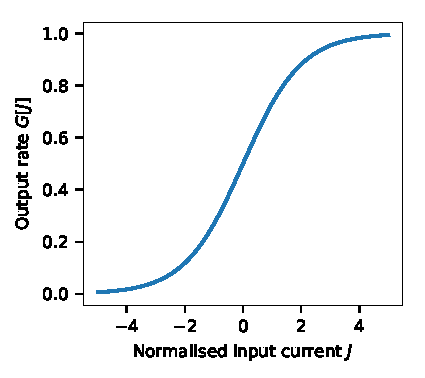
\includegraphics{media/nonlinearity_logistic.pdf}%
		\caption{Logistic function}%
		\label{fig:artificial_neurons_logistic}
	\end{subfigure}%
	\begin{subfigure}{0.5\textwidth}%
		\centering%
		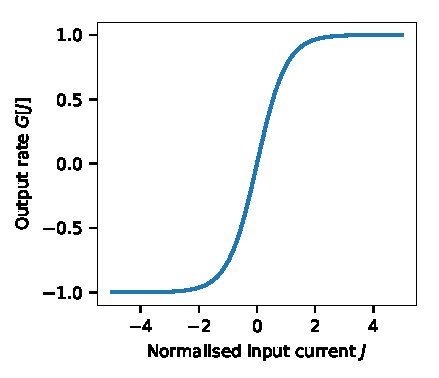
\includegraphics{media/nonlinearity_tanh.pdf}%
		\caption{Hyperbolic Tangent}%
		\label{fig:artificial_neurons_tanh}
	\end{subfigure}
	\caption{Overview of some neural response functions used in artifical neural networks. \CodeLink{lecture_02/media/code/neuron_nonlinearities.ipynb}}
	\label{fig:artificial_neurons}
\end{figure}

\paragraph{The Rectified Linear Unit (ReLU)}
This non-linearity is defined as $G[J] = \max\{0, J\}$ (\cref{fig:artificial_neurons_relu}). This is actually a reasonable substitute for the LIF rate approximation, especially in those cases where $\tau_\mathrm{RC}$ is large (cf.~\cref{fig:lif_neuron_rate}). Interestingly, this function has experienced a resurgence of interest with the recent developments in \enquote{deep learning}.

\paragraph{The Softplus or Smooth ReLU function}
This non-linearity is defined as $G[J] = \log(1 + \exp(J))$ (\cref{fig:artificial_neurons_smooth_relu}). The overall shape is the same as for the rectified linear unit, yet the sharp \enquote{kink} at $J = 0$ is smoothed out. In a neural setting, one finds such smoothing when superimposing noise onto the input current $J$. The Smooth ReLU function is hence vaguely comparable to rate approximations of the LIF neuron that take noise into account \cite{hunsberger2015spiking}.

\paragraph{The Logistic Activation function}
This function is defined as $G[J] = \frac{1}{1 + e^{-J}}$ (\cref{fig:artificial_neurons_logistic}). It is a so called \emph{sigmoid} function (because of the \enquote{S} shape). If we wanted to interpret this activation function from a biological standpoint, we could say that this function captures the smooth onset observed in a noisy system, as well as the saturation effect we see in the LIF rate approximation. The Logistic Activation Function and the Hyperbolic Tangent function are among the most widely used non-linearities in machine learning (at least before the ReLU took over).

\paragraph{The Hyperbolic Tangent function}
This function is defined as $G[J] = \tanh(J) = \frac{e^J - e^{-J}}{e^J + e^{-J}}$ (\cref{fig:artificial_neurons_tanh}) and is similar in shape to the logistic activation function -- one difference to all the other functions we looked at so far is that we have negative rates -- this is something that matters very little in machine learning, but would definitively not be a valid response function for our purposes. This emphasizes again that artifical neurons are not at all designed with biological plausibility in mind.


%Embedded into the cell membrane are special proteins that act as gateways for matter that flows into or out of the cell. These proteins may either actively transport matter, or passively act as a filter that only lets certain kinds of matter through (\cref{fig:neuron_sketch_membrane}).

%\subsection{Reducing Neurons to a Single Point}

%\begin{figure}[t]
%	\centering%
%	\begin{subfigure}{0.5\textwidth}%
%		\centering%
%		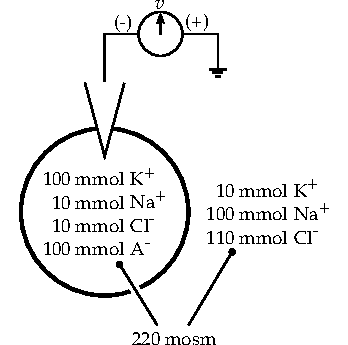
\includegraphics{media/neuron_channel_a.pdf}%
%		\caption{Neuron in resting state}%
%		\label{fig:neuron_channel_a}
%	\end{subfigure}%
%	\begin{subfigure}{0.5\textwidth}%
%		\centering%
%		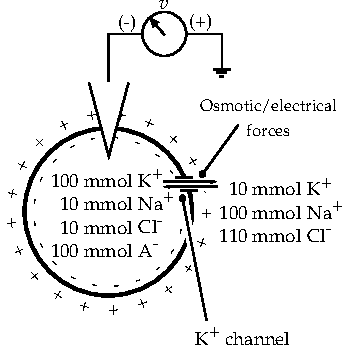
\includegraphics{media/neuron_channel_b.pdf}%
%		\caption{After adding a selectively permeable ion channel}%
%		\label{fig:neuron_channel_b}
%	\end{subfigure}
%	\caption{Effects of a semipereable ion channel on the neural potential. \textbf{(a)} The neuron is in a resting state, and the intra- and extra-cellular fluid is electrectically neutral. \textbf{(b)} Once we add a semi-permeable ion channel, a new equilibrium state will be created by countering osmotic and electrical forces. From \cite{stoeckel2015design}, adapted from \cite{reichert2000neurobiologie}.}
%\end{figure}

%The intra- and extra-cellular fluids contain electrically charged particles, mostly ions and some complex electrically charged molecules. To simplify things a little, let's assume that the fluid on the in- and outside of the cell is homogeneous, i.e.~has the same properties everywhere. Correspondingly, we can collapse the entire elaborately shaped neuron into a small sphere -- the only thing that matters when we measure ion concentrations or electrical potentials is whether we're on the inside or the outside of the cell.

%When we measure ion concentrations of the intra-cellular fluid and the extra-cellular fluid, we find that both fluids are electrically neutral, yet contain different concentrations of ions.\footnote{Special \enquote{ion pump} proteins in the cell membrane ensure over long periods of time that this mixture approximately stays the same.} The cells being electrically \emph{neutral} means, that there is nothing interesting  (\cref{fig:neuron_channel_a}).


%\subsection{Spike Production: The Hodgkin Huxley Neuron Model}

%\section{The Leaky Integrate and Fire Neuron Model}

%\section{Artifical Neurons}


\printbibliography

\end{document}
